\documentclass[tikz,border=1pt]{standalone}
\usepackage[T1]{fontenc}
\usepackage{mathptmx}
\renewcommand{\ttdefault}{pcr}
\usepackage{tikz}
\usepackage{siunitx}
\usepackage{amssymb}
\sisetup{group-separator={,},group-minimum-digits=4}
\usetikzlibrary{positioning,arrows.meta,calc,fit,backgrounds,shapes.misc}
% palette shared with make_figs.py
\definecolor{ink}{HTML}{0B0B0B}
\definecolor{ink2}{HTML}{52514E}
\definecolor{muted}{HTML}{8A8984}
\definecolor{rule}{HTML}{E6E5E1}
\definecolor{paper}{HTML}{F7F6F3}
\definecolor{good}{HTML}{1BAF7A}
\definecolor{kh}{HTML}{E34948}
\definecolor{ball}{HTML}{EDA100}
\definecolor{lof}{HTML}{2A78D6}
\definecolor{agent}{HTML}{3D3A6B}
\definecolor{agentbg}{HTML}{EEEDF6}
\definecolor{serverbg}{HTML}{EAF3EE}
\tikzset{
  >={Stealth[length=2.2mm,width=1.6mm]},
  box/.style={draw=ink2, line width=0.5pt, rounded corners=2pt, fill=white, align=center, inner sep=3pt, font=\footnotesize},
  chip/.style={draw=ink2, line width=0.4pt, rounded corners=1.5pt, fill=white, font=\scriptsize\ttfamily, inner xsep=3pt, inner ysep=2pt, minimum height=4.2mm},
  region/.style={draw=muted, line width=0.5pt, dashed, rounded corners=4pt, inner sep=6pt},
  lab/.style={font=\scriptsize, text=ink2, align=center},
  flow/.style={->, line width=0.6pt, draw=ink2},
  ret/.style={->, line width=0.6pt, draw=ink2, densely dashed},
  bubble/.style={draw=ink2, line width=0.5pt, rounded corners=6pt, fill=paper, align=left, inner sep=4pt, font=\footnotesize},
  num/.style={circle, fill=ink, text=white, font=\tiny\bfseries, inner sep=0.8pt, minimum size=3.4mm},
}

\definecolor{p1}{HTML}{F4F4F2}\definecolor{p1d}{HTML}{6B6A66}
\definecolor{p3}{HTML}{EAF5EE}\definecolor{p3d}{HTML}{3E8E5E}
\definecolor{p4}{HTML}{EAF1FA}\definecolor{p4d}{HTML}{2A5FA8}
\tikzset{
  panel/.style={draw=#1, line width=0.7pt, rounded corners=4pt, minimum height=60mm, anchor=north west},
  ptitle/.style={font=\footnotesize\bfseries, text=ink, anchor=west, inner sep=0},
  stp/.style={draw=agent!45, fill=white, rounded corners=2pt, minimum width=36mm, minimum height=4.6mm, anchor=north west, font=\scriptsize, align=left, text width=34mm, inner sep=1.5pt},
  sub/.style={draw=p3d!60, fill=white, rounded corners=2.5pt, text width=31.5mm, anchor=north west, font=\scriptsize, align=left, inner sep=2pt},
  sn/.style={circle, fill=agent, text=white, font=\tiny\bfseries, inner sep=0.6pt, minimum size=3mm},
}
% simple vector icons
\newcommand{\person}[1]{\begin{scope}[shift={#1}]\fill[p1d] (0,1.15mm) circle (0.95mm);\fill[p1d] (-1.75mm,-1.7mm) -- (-1.75mm,-0.9mm) arc[start angle=180,end angle=0,x radius=1.75mm,y radius=1.1mm] -- (1.75mm,-1.7mm) -- cycle;\end{scope}}
\newcommand{\robot}[1]{\begin{scope}[shift={#1}]\fill[agent,rounded corners=0.6mm] (-1.8mm,-1.3mm) rectangle (1.8mm,1.3mm);\fill[white] (-0.75mm,0.2mm) circle (0.4mm) (0.75mm,0.2mm) circle (0.4mm);\draw[agent,line width=0.5pt] (0,1.3mm) -- (0,2.1mm);\fill[agent] (0,2.2mm) circle (0.35mm);\end{scope}}
\newcommand{\server}[1]{\begin{scope}[shift={#1}]\foreach \y in {-1.3,0,1.3}{\fill[p3d,rounded corners=0.3mm] (-1.9mm,\y mm-0.55mm) rectangle (1.9mm,\y mm+0.55mm);\fill[white] (1.2mm,\y mm) circle (0.22mm);}\end{scope}}
\newcommand{\chart}[1]{\begin{scope}[shift={#1}]\draw[p4d,line width=0.5pt,rounded corners=0.3mm] (-2mm,-1.5mm) rectangle (2mm,1.5mm);\draw[p4d,line width=0.6pt] (-1.4mm,-0.9mm) -- (-0.4mm,0.1mm) -- (0.3mm,-0.4mm) -- (1.4mm,0.9mm);\end{scope}}
\begin{document}
\begin{tikzpicture}
% ---------------- panel 1
\node[panel=p1d, fill=p1, minimum width=29mm] (P1) at (0,0) {};
\person{(4mm,-5.2mm)}
\node[ptitle, text width=21mm, align=left] at (7.5mm,-5mm) {Process engineer\\[-1pt]{\scriptsize\mdseries\color{ink2}plain language}};
\node[bubble, fill=white, text width=23mm, anchor=north west, font=\scriptsize\itshape, inner sep=2.5pt] at (1.3mm,-11.5mm) {%
``Find the lowest-spatter defect-free parameters that stay at least 15\,\textmu m above the lack-of-fusion depth and at least 0.1 below the keyhole $D/W$ threshold.''};
% ---------------- panel 2
\node[panel=agent, fill=agentbg, minimum width=40mm] (P2) at (33mm,0) {};
\robot{(37mm,-5.2mm)}
\node[ptitle] at (40.5mm,-5mm) {AgentAM {\scriptsize\mdseries\color{ink2}(LLM agent)}};
\foreach \i/\t in {1/Read the request, 2/Choose a tool and its inputs, 3/Call the MCP server, 4/Check limits and margins, 5/Report returned values only}{
  \node[stp] (s\i) at (35mm,{-10mm-(\i-1)*5.6mm}) {\hspace{4mm}\t};
  \node[sn] at ($(s\i.west)+(2.3mm,0)$) {\i};
}
\node[anchor=north west, inner sep=0] (code) at (35mm,-39.5mm) {\setlength{\fboxsep}{2pt}\fcolorbox{agent!45}{white}{\parbox{35mm}{\scriptsize\ttfamily\raggedright
mcp\_find\_robust(\\
\ min\_depth\_margin=15,\\
\ min\_dw\_margin=0.1)}}};
\node[lab, anchor=north west, font=\tiny] at (35mm,-50.5mm) {call made by the agent (benchmark C15)};
% ---------------- panel 3
\node[panel=p3d, fill=p3, minimum width=36mm] (P3) at (82mm,0) {};
\server{(86mm,-5.2mm)}
\node[ptitle] at (89.5mm,-5mm) {MCP tool server {\scriptsize\mdseries\color{ink2}(local)}};
\node[sub] (a) at (84.2mm,-10mm) {\textbf{Surrogate models}\\{\color{ink2}polynomial; 279 CFD tracks}\\melt pool $D$, $W$, $L$;\; spatter volume};
\node[sub] (b) at ($(a.south west)+(0,-1.5mm)$) {\textbf{Defect classifier}\\
\textcolor{kh}{$\blacksquare$}\,keyhole\hfill $D/W>1.25$\\
\textcolor{lof}{$\blacksquare$}\,lack of fusion\hfill $D<137$\,\textmu m\\
\textcolor{ball}{$\blacksquare$}\,balling\hfill $2.35<L/W<3.7$\\
\textcolor{good}{$\blacksquare$}\,good\hfill otherwise};
\node[sub] (c) at ($(b.south west)+(0,-1.5mm)$) {\textbf{Scans and optimizers}\\$P$--$V$ scans;\; constrained and margin-aware search};
% ---------------- panel 4
\node[panel=p4d, fill=p4, minimum width=43mm] (P4) at (122mm,0) {};
\chart{(126.3mm,-5.2mm)}
\node[ptitle] at (129.8mm,-5mm) {Result to the engineer};
\node[anchor=north west, inner sep=0] (map) at (124mm,-8.5mm) {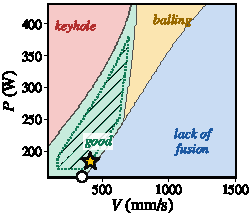
\includegraphics[width=36mm]{overview_map_m.pdf}};
\node[anchor=north west, fill=white, draw=p4d!50, rounded corners=2.5pt, text width=38mm, font=\scriptsize, align=left, inner sep=2pt] (ans) at (123.5mm,-40mm) {%
\textcolor{ball!90!black}{$\bigstar$}\,\textbf{184\,W, 411\,mm/s}\;\textcolor{good}{$\blacksquare$}\,good\\
spatter \num{55470}\,\textmu m$^3$;\; $D=152$\,\textmu m\\
{\color{ink2}nearest: lack of fusion, +15\,\textmu m}\\[1pt]
$\circ$\,plain optimum 160\,W, 349\,mm/s: +6.7\,\textmu m, at range edge\\[1pt]
\textbf{margins cost +39.8\% spatter}};
% ---------------- arrows
\draw[flow, line width=0.8pt] (P1.east|-0,-30mm) -- (P2.west|-0,-30mm);
\draw[flow, line width=0.8pt] ($(P2.east)+(0,6mm)$) -- node[lab, above, font=\tiny]{tool call} ($(P3.west)+(0,6mm)$);
\draw[ret, line width=0.8pt] ($(P3.west)+(0,-2mm)$) -- node[lab, below, font=\tiny]{JSON} ($(P2.east)+(0,-2mm)$);
\draw[flow, line width=0.8pt] (P3.east) -- (P4.west|-P3.east);
% ---------------- evaluation bar
\node[anchor=north west, draw=rule, fill=paper, rounded corners=3pt, minimum width=165mm, minimum height=8mm, inner sep=0] (E) at (0,-62mm) {};
\node[anchor=west, font=\footnotesize\bfseries] at (2mm,-66mm) {Evaluation (agent layer)};
\foreach \x/\t in {50/{145 prompts, 725 runs}, 80/{inputs passed: \textbf{98.5\%}}, 112/{constraints met: \textbf{all}}, 146/{without tools: \textbf{80\%} fabricated}}{
  \node[anchor=center, font=\scriptsize] at (\x mm,-66mm) {\t};}
\foreach \x in {37,65,96,128}{\draw[rule, line width=0.6pt] (\x mm,-63.5mm) -- (\x mm,-68.5mm);}
\end{tikzpicture}
\end{document}
